\documentclass[12pt]{article}

\usepackage[margin=1in]{geometry}
\usepackage{amsmath, amsthm}
\usepackage{amssymb}
\usepackage{graphicx}
\usepackage{times}
% \usepackage{subcaption}
\usepackage[colorlinks=true, linkcolor=black, citecolor=black, urlcolor=black]{hyperref}


\title{CSCI 5352: Homework 4}
\author{
    Zachary Caterer$^{1,2,3}$ \\
    \small $^1$Department of Computer Science, University of Colorado Boulder \\
    \small $^2$Department of Chemical and Biological Engineering, University of Colorado Boulder \\
    \small $^3$Interdisciplinary Quantitative Biology Program, University of Colorado Boulder
}
\date{\today}

\begin{document}

\maketitle

\subsection*{Collaborators}
I worked with the following people on this assignment:

\begin{itemize}
    \item Ben Braun
    \item Logan Barrios
    \item Luis Paez
    \item Michael Luzadder
    \item Pedro Lemos
\end{itemize}

\section*{Problem 1}
\[
M = 
\begin{bmatrix}
\text{Region} & \text{Northeast} & \text{Midwest} & \text{South} & \text{West} & \text{Canada} \\
\text{Northeast} & 0.119 & 0.053 & 0.074 & 0.055 & 0.022 \\
\text{Midwest} & 0.031 & 0.067 & 0.061 & 0.026 & 0.011 \\
\text{South} & 0.025 & 0.027 & 0.083 & 0.024 & 0.006 \\
\text{West} & 0.049 & 0.033 & 0.043 & 0.073 & 0.011 \\
\text{Canada} & 0.006 & 0.005 & 0.005 & 0.005 & 0.085
\end{bmatrix}
\]

\[
\begin{bmatrix}
  \text{Region}    &   \text{Edge Fraction} (e_r)  & \text{Row Sum} (a_r)    &   Q_r     \\
  \text{Northeast} &        0.238                  &   0.553                 &  -0.067809\\
  \text{Midwest}   &        0.134                  &   0.381                 &  -0.011161\\
  \text{South}     &        0.166                  &   0.431                 &  -0.019761\\
  \text{West}      &        0.146                  &   0.392                 &  -0.007664\\
  \text{Canada}    &        0.170                  &   0.241                 &   0.111919\\
\end{bmatrix}
\]

\[
 \text{Total modularity } Q: 0.005524000000000057
\]

The modularity: $Q = 0.00552$ is very close to zero, indicating that there is very little assortative mixing by region. This means that professors are not significantly more likely to stay within the same geographic region when transitioning from a PhD institution to a faculty position. Canada has the largest positive $Q_r$, suggesting that there is a relatively stronger tendency for movement to remain within Canada. The Northeast has the most negative $Q_r$, indicating that faculty movement out of the Northeast is relatively high compared to how many stay within the region. The overall low modularity suggests that the different regions are strongly interconnected, with no strong preference for remaining within the same geographic region.

\section*{Problem 2}

\subsection*{Part A}
Modularity is defined as

\[
Q = \frac{1}{2m}\sum_{ij}(A_{ij} - \frac{k_i k_j}{2m}) \delta(c_i, c_j) = \sum_u (e_{uu} - a_u^2)
\]

Where $e_{uu}$ for each group
\[
e_1 = \frac{g-1}{n-1}, \quad e_2 = \frac{(n-g) - 1}{n-1}
\] 

\[
\implies \sum_u e_{uu} = \frac{g-1}{n-1} + \frac{(n-g) - 1}{n-1} = \frac{n-2}{n-1}
\]

And $a_u$ for each group
\[
a_1 = \frac{2(g-1) +1}{2(n-1)} = \frac{2g-1}{2{n-1}}
\]

\[
a_2 = \frac{2(n-g-1)+1}{2(n-1)} = \frac{2(n-g)-1}{2(n-1)}
\]

\[
\implies \sum a_u^2 = a_1^2 + a_2^2 = \left( \frac{2g-1}{2(n-1)}\right) ^2 + \left( \frac{2(n-g)-1}{2(n-1)}\right) ^2
\]

\[
= \frac{8g^2 + 4n^2 - 8ng - 4n + 2}{4(n-1)^2} 
\]

\[
\implies Q = \frac{n-2}{n-1} - \frac{8g^2 + 4n^2 - 8ng - 4n + 2}{4(n-1)^2} 
\]


\[
= \frac{-8n + 6 -8g^2 + 8ng}{4(n-1)^2}  = \frac{3 - 4n + 4gn - 4g^2}{2(n - 1)^2} \quad \blacksquare
\]

\subsection*{Part B}
If we treat $Q$ as a function of $g$, we can find the maximum by taking the derivative with respect to $g$ and setting it equal to zero:

$$
\frac{dQ}{dg} = \frac{2n}{(n-1)^2} - \frac{4g}{(n-1)^2} = 0
$$

And solving for $g$: $2n = 4g \implies g = \frac{n}{2}$

And to prove that this is a maximum, we can take the second derivative:

$$
\frac{d^2Q}{dg^2} = -\frac{4}{(n-1)^2} < 0
$$

Since the second derivative is negative, this confirms that $g = \frac{n}{2}$ is a maximum. Thus, the optimal number of groups is $g = \frac{n}{2}$.

\begin{flushright}
  \(\blacksquare\)
\end{flushright}

\section*{Problem 3}
\subsection*{Part A}

We are given a network with 9 nodes and a 2-group partition:

- Group 1: ${1, 2, 8, 9, 7}$
- Group 2: ${3, 4, 5, 6}$

The edge list:

$$
edges = [(1, 2), (1, 3), (1, 6), (1, 7), (1, 8), (1, 9), (3, 4), (3, 6), (4, 6), (5, 6)]
$$

The mixing matrix $M$ is a $2 \times 2$ matrix where:

$$
M_{rs} = \frac{e_{rs}}{n_{rs}} \quad \text{where} \quad e_{rs} = \sum_{i<j}^n A_{ij}\delta_{r,z_i}\delta_{s,z_j} \quad \text{and} \quad n_{rs} = \sum_{i<j}^n \delta_{r,z_i}\delta_{s,z_j}
$$


The log-likelihood function for SBM:

$$
\ln \mathcal{L} = \sum_{r,s} e_{rs} \ln M_{rs} + (n_{rs} - e_{rs})\ln(\frac{n_{rs} - e_{rs}}{n_{rs}})
$$

(i) Maximum Likelihood Mixing Matrix
$$
M = \begin{bmatrix} \frac{4}{10} & \frac{2}{20} \\ -- & \frac{4}{6} \end{bmatrix}
$$

(ii) Log-likelihood
$$
\ln \mathcal{L} = (4 \ln \frac{4}{10} + 6\ln \frac{6}{10}) + (2 \ln \frac{2}{20} + 18\ln \frac{18}{20}) + (4 \ln \frac{4}{6} + 2\ln \frac{2}{6})  \approx -17.051
$$

\subsection*{Part B}

We are given a network with 9 nodes and a 2-group partition same as in Problem 3(a):

The mixing matrix $\omega$ is a $2 \times 2$ matrix where:

$$
\omega_{rs} = \sum_{i,j=1}^n A_{ij}\delta_{z_i,r}\delta_{z_j,s} \quad \text{and} \quad K_r = \sum_s \omega_{rs} = \sum_i k_i \delta_{z_i, r}
$$

The log-likelihood function for DC-SBM:

$$
\ln \mathcal{L} = \sum_{rs} \omega_{rs} ln \frac{\omega_{rs}}{K_r K_s}
$$


(i) DC-SBM Mixing Matrix
$$
\omega = \begin{bmatrix} & O & T & K_r \\ O & 8 & 2 & 10 \\ T & 2 & 8 & 10\end{bmatrix}
$$

(ii) log-likelihood
$$
\ln \mathcal{L} = \sum_{rs} \omega_{rs} \ln \frac{\omega_{rs}}{K_r K_s} 

= (8 \ln \frac{8}{10 \times 10}) + (2 \ln \frac{2}{10 \times 10}) + (2 \ln \frac{2}{10 \times 10}) + (8 \ln \frac{8}{10 \times 10})

\approx -56.060
$$

\subsection*{Part C}

Comparing the log-likelihoods of both models:

SBM Log-Likelihood: $\ln \mathcal{L} \approx -17.05$

DC-SBM Log-Likelihood: $\ln \mathcal{L} \approx -56.06$

Since the log-likelihood is significantly lower for the Degree-Corrected Stochastic Block Model (DC-SBM), this suggests that SBM better captures the structure of the observed network. This is likely because DC-SBM accounts for degree heterogeneity, which the standard SBM does not. Thus, the DC-SBM is less likely to have generated the observed network.

\section*{Problem 4}
\subsection*{Part A}
\begin{figure}[h] 
  \centering 
  \begin{minipage}{0.48\textwidth} 
      \centering 
      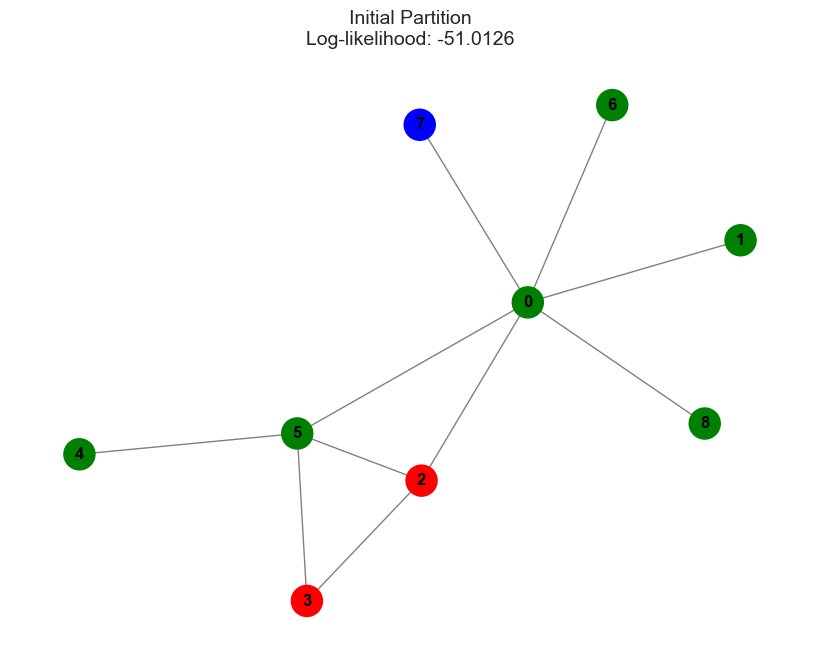
\includegraphics[width=\textwidth]{../figures/4a_initial_partition.png} 
  \end{minipage} 
  \hfill 
  \begin{minipage}{0.48\textwidth} 
      \centering 
      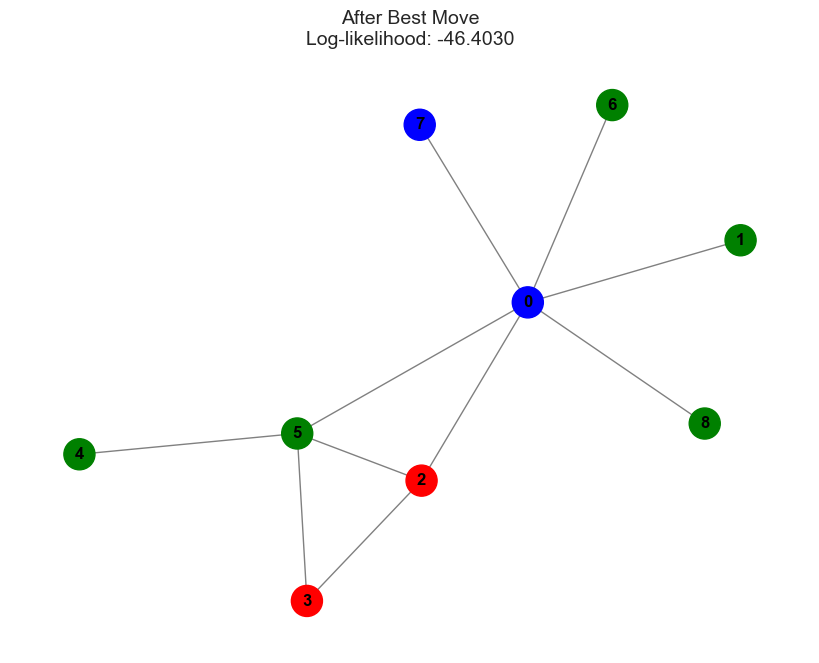
\includegraphics[width=\textwidth]{../figures/4a_best_move.png} 
  \end{minipage} 
  \caption{(Left) The input graph $G$ with its initial partition $z_t$, where node labels indicate group assignments, and the log-likelihood is computed under the Degree-Corrected Stochastic Block Model (DC-SBM). (Right) The graph after applying the best move found by makeAMove(), updating the partition to maximize the log-likelihood $\mathcal{L}_*$
    while keeping frozen nodes unchanged.}
  \label{fig:4a_best_move} 
\end{figure}

\subsection*{Part B}
\begin{figure}[h] 
  \centering 
  \begin{minipage}{0.48\textwidth} 
      \centering 
      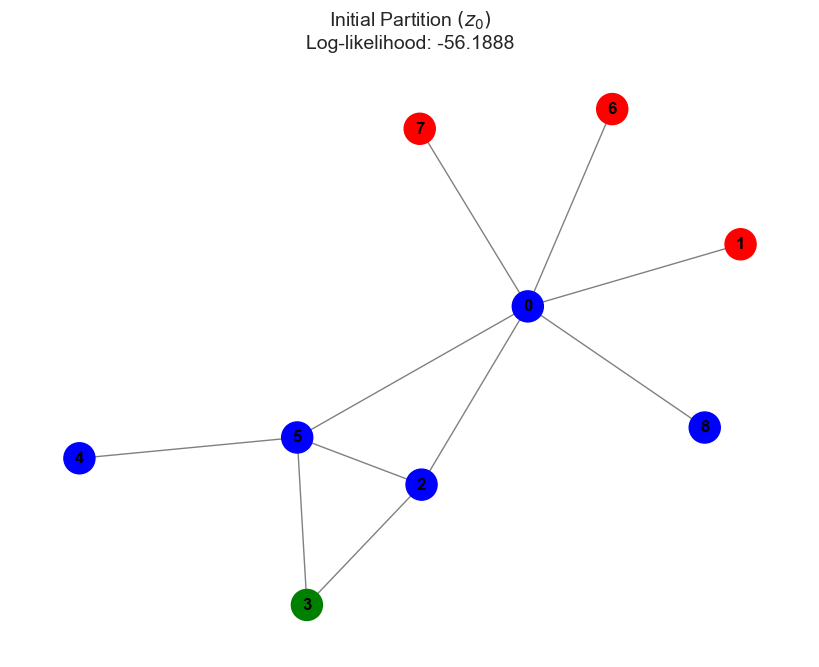
\includegraphics[width=\textwidth]{../figures/4b_initial_partition.png} 
  \end{minipage} 
  \hfill 
  \begin{minipage}{0.48\textwidth} 
      \centering 
      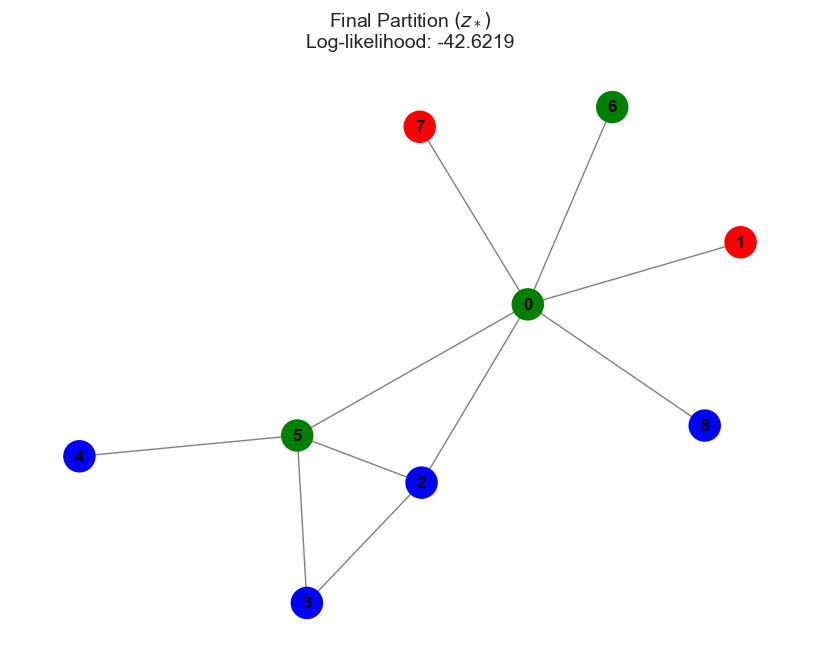
\includegraphics[width=\textwidth]{../figures/4b_final_partition.png} 
  \end{minipage} 
  \caption{The input graph $G$ with its initial partition $z_0$, where node labels indicate group assignments, and the log-likelihood is computed under the Degree-Corrected Stochastic Block Model (DC-SBM). (Right) The graph after completing one full phase of the algorithm, showing the final partition $z_*$ that maximizes the log-likelihood $\mathcal{L}_*$.}
  \label{fig:4b} 
\end{figure}

\begin{figure}
    \centering
    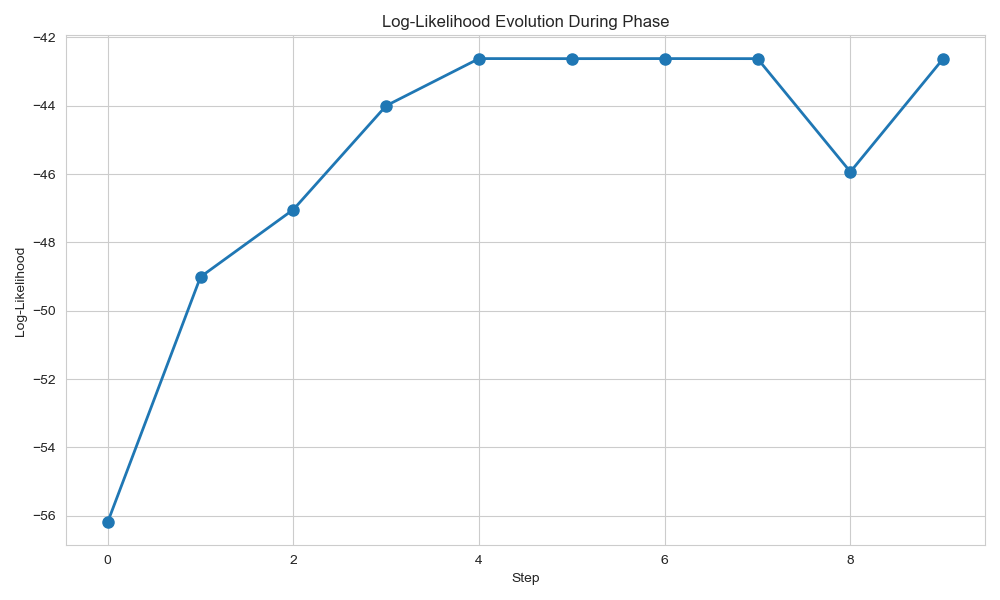
\includegraphics[width=0.5\textwidth]{../figures/4b_likelihood_evolution.png}
    \caption{The evolution of the log-likelihood $\ell_t$ over the course of the phase, illustrating the algorithm’s progression as nodes are sequentially frozen and reassigned to optimize the partition.}
    \label{fig:4b_modularity}
\end{figure}

Please refer to Figures 2 for the initial and final partitions, and Figure 3 for the log-likelihood evolution.

\subsection*{Part C}
\begin{figure}[h] 
  \centering 
  \begin{minipage}{0.48\textwidth} 
      \centering 
      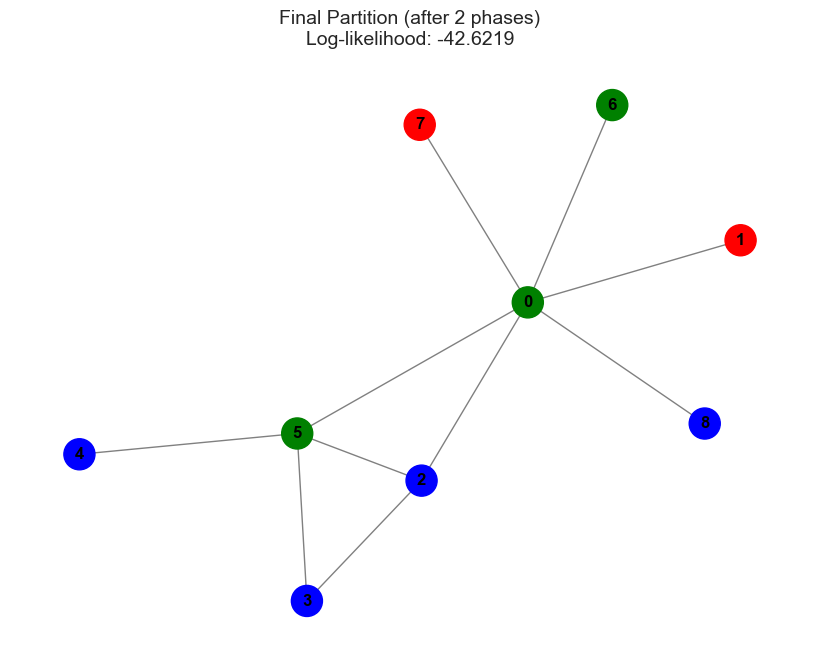
\includegraphics[width=\textwidth]{../figures/4c_final_partition.png} 
  \end{minipage} 
  \hfill 
  \begin{minipage}{0.48\textwidth} 
      \centering 
      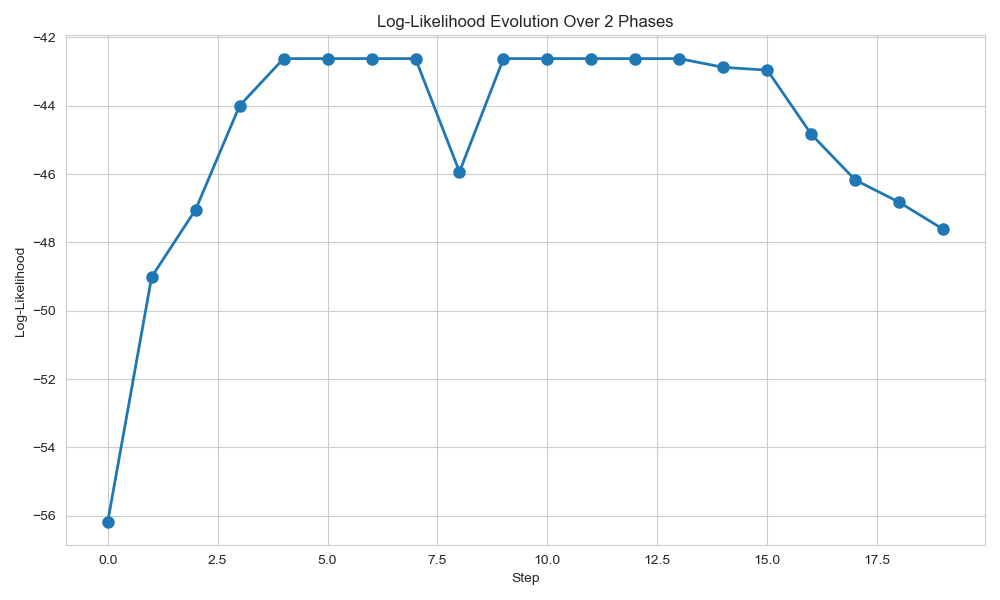
\includegraphics[width=\textwidth]{../figures/4c_likelihood_evolution.png} 
  \end{minipage} 
  \caption{(Left) The final partition $z_*$ of the graph $G$ obtained after running the full locally greedy heuristic (fitDCSBM()), where node labels indicate group assignments that maximize the Degree-Corrected Stochastic Block Model (DC-SBM) log-likelihood $\mathcal{L}_*$. (Right) The evolution of the log-likelihood $\ell_t$ over the course of all phases, illustrating the improvement in partition quality as the algorithm progresses toward convergence then falls again after step 15.}
  \label{fig:4a_best_move} 
\end{figure}

\[
\omega \begin{bmatrix}
  0. & 4. & 1. \\
  4. & 0. & 5. \\
  1. & 5. & 0. \\
\end{bmatrix}
\]

\[
\vec{K} = \begin{bmatrix}
  5. \\
  9. \\
  6. \\
\end{bmatrix}
\]

It takes about 4 steps to reach the maximum of the log-likelihood, takes a dip around step 8 in phase one, and in the second phase it begins to decrease after step 15 (Fig 4.) I achieved a log-likelihood of $\approx -42.623$ which is shown in Figure 4.


\subsection*{Part D}

\begin{figure}[h] 
  \centering 
  \begin{minipage}{0.48\textwidth} 
      \centering 
      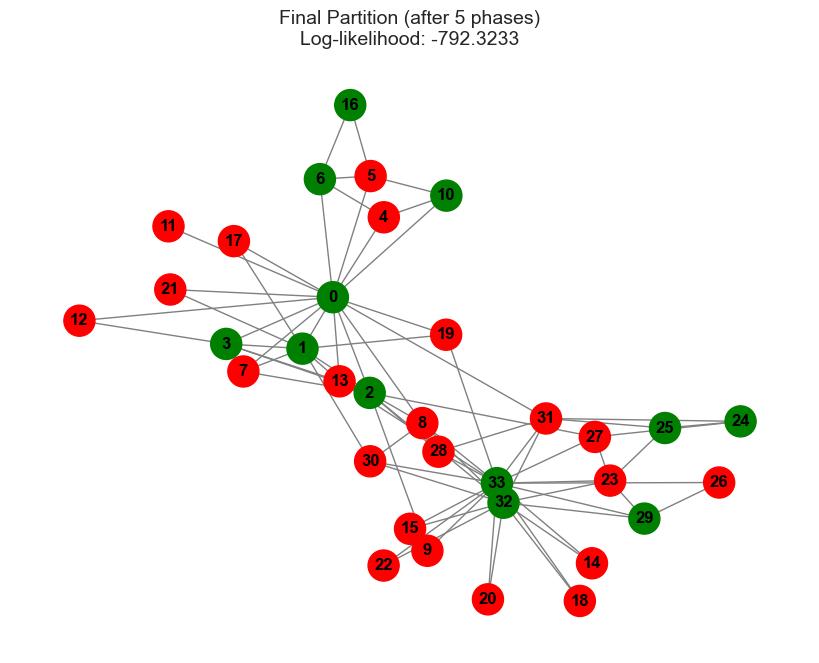
\includegraphics[width=\textwidth]{../figures/4d_final_partition.png} 
  \end{minipage} 
  \hfill 
  \begin{minipage}{0.48\textwidth} 
      \centering 
      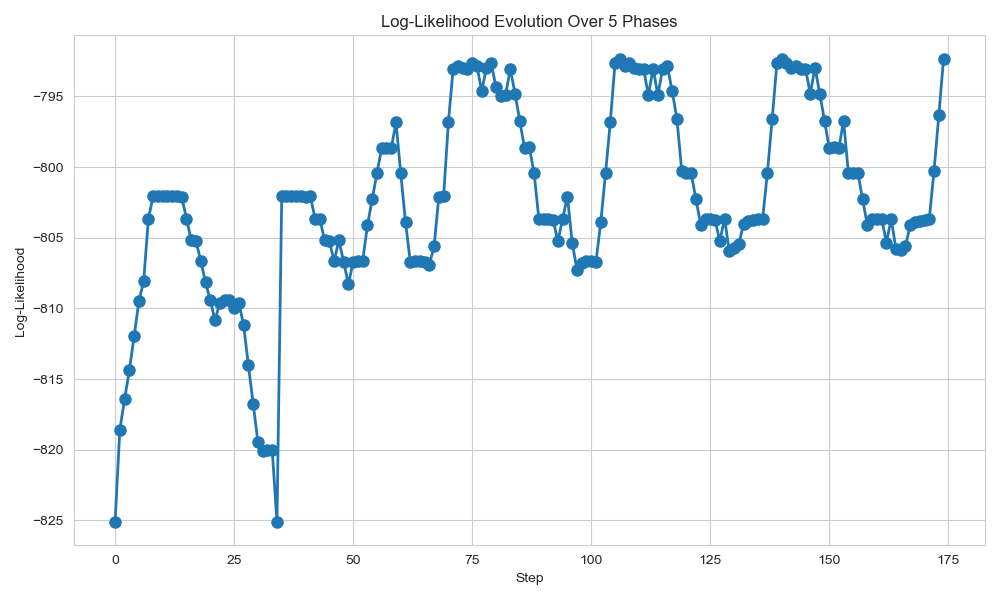
\includegraphics[width=\textwidth]{../figures/4d_likelihood_evolution.png} 
  \end{minipage} 
  \caption{(Left) The best partition $z_*$ of the Zachary Karate Club network obtained after multiple runs of fitDCSBM(), successfully recovering the optimal $c = 2$ group structure described in the lecture notes. Node labels indicate final group assignments that maximize the Degree-Corrected Stochastic Block Model (DC-SBM) log-likelihood $\mathcal{L}_*$. (Right) The evolution of the log-likelihood $\ell_t$ over the best run, illustrating how the partition improved over successive phases.}
  \label{fig:4a_best_move} 
\end{figure}

\[
\omega = \begin{bmatrix}
  3  & 61 \\
  61 & 14 \\
\end{bmatrix}
\]

\[
\vec{K} = \begin{bmatrix}
  67 \\
  89 \\
\end{bmatrix}
\]


My final partition log-likelihood was approximately \(-792.323\), as shown in Figure 5. The algorithm reached a similar log-likelihood around cycle 3, after which the log-likelihood oscillated between \(\approx -807\) and \(\approx -792\) over subsequent cycles. This suggests that stopping the multi-run process after three phases would yield nearly the same outcome as running for five. However, the final partition I obtained does not exactly match the original partition of the Zachary Karate Club network. This indicates that while the algorithm converged to a high-likelihood solution, some variability remains in the partitions found across different runs.

\section*{Problem 5}

I read the paper "Projecting the transmission dynamics of SARS-CoV-2 through the postpandemic period" by Kissler et al. The research question in this paper focuses on projecting the transmission dynamics of SARS-CoV-2 in the post-pandemic period. The authors aimed to understand how seasonal variation, immunity duration, and cross-immunity with other coronaviruses might influence future outbreaks. They sought to determine whether SARS-CoV-2 would persist through recurrent outbreaks, be eradicated, or transition into an endemic seasonal virus, and they explored the potential need for long-term interventions such as social distancing.

To address this question, the authors developed a mathematical model based on historical data from human coronaviruses OC43 and HKU1. They incorporated factors like immunity waning, cross-immunity, and seasonal transmission patterns. The model was used to simulate different scenarios for SARS-CoV-2 transmission through 2025, analyzing how various intervention strategies, including intermittent social distancing, might help manage outbreaks while preventing healthcare system overload.

One of the paper’s strengths is its exceptional use of figures, which are well-crafted and curated to communicate the scope of the study clearly. The authors maintained consistent themes and colors across their visuals, which reflects deliberate effort and enhances comprehension. I often assess a paper’s figures first to get an intuitive sense of its content, and in this case, the figures alone provide a clear representation of the study’s methodology and findings. However, the study could have improved by incorporating more real-world validation of its model through emerging empirical data on SARS-CoV-2 immunity. Additionally, exploring regional differences in seasonality and transmission could have strengthened the analysis. Future extensions could include refining the model with updated serological data, integrating vaccine impact, or assessing new therapeutic strategies to mitigate recurrent outbreaks.


\end{document}